\documentclass[11pt,a4paper,openany]{memoir}\usepackage[]{graphicx}\usepackage[]{color}
%% maxwidth is the original width if it is less than linewidth
%% otherwise use linewidth (to make sure the graphics do not exceed the margin)
\makeatletter
\def\maxwidth{ %
  \ifdim\Gin@nat@width>\linewidth
    \linewidth
  \else
    \Gin@nat@width
  \fi
}
\makeatother

\definecolor{fgcolor}{rgb}{0.345, 0.345, 0.345}
\newcommand{\hlnum}[1]{\textcolor[rgb]{0.686,0.059,0.569}{#1}}%
\newcommand{\hlstr}[1]{\textcolor[rgb]{0.192,0.494,0.8}{#1}}%
\newcommand{\hlcom}[1]{\textcolor[rgb]{0.678,0.584,0.686}{\textit{#1}}}%
\newcommand{\hlopt}[1]{\textcolor[rgb]{0,0,0}{#1}}%
\newcommand{\hlstd}[1]{\textcolor[rgb]{0.345,0.345,0.345}{#1}}%
\newcommand{\hlkwa}[1]{\textcolor[rgb]{0.161,0.373,0.58}{\textbf{#1}}}%
\newcommand{\hlkwb}[1]{\textcolor[rgb]{0.69,0.353,0.396}{#1}}%
\newcommand{\hlkwc}[1]{\textcolor[rgb]{0.333,0.667,0.333}{#1}}%
\newcommand{\hlkwd}[1]{\textcolor[rgb]{0.737,0.353,0.396}{\textbf{#1}}}%

\usepackage{framed}
\makeatletter
\newenvironment{kframe}{%
 \def\at@end@of@kframe{}%
 \ifinner\ifhmode%
  \def\at@end@of@kframe{\end{minipage}}%
  \begin{minipage}{\columnwidth}%
 \fi\fi%
 \def\FrameCommand##1{\hskip\@totalleftmargin \hskip-\fboxsep
 \colorbox{shadecolor}{##1}\hskip-\fboxsep
     % There is no \\@totalrightmargin, so:
     \hskip-\linewidth \hskip-\@totalleftmargin \hskip\columnwidth}%
 \MakeFramed {\advance\hsize-\width
   \@totalleftmargin\z@ \linewidth\hsize
   \@setminipage}}%
 {\par\unskip\endMakeFramed%
 \at@end@of@kframe}
\makeatother

\definecolor{shadecolor}{rgb}{.97, .97, .97}
\definecolor{messagecolor}{rgb}{0, 0, 0}
\definecolor{warningcolor}{rgb}{1, 0, 1}
\definecolor{errorcolor}{rgb}{1, 0, 0}
\newenvironment{knitrout}{}{} % an empty environment to be redefined in TeX

\usepackage{alltt}

\setsecnumdepth{subsection}
\maxtocdepth{subsection}
\raggedbottom
\setulmarginsandblock{1.5cm}{1.5cm}{*}
\setlrmarginsandblock{4cm}{4cm}{*}

\usepackage[hidelinks]{hyperref}
\usepackage{geometry}
\usepackage{setspace}
\usepackage{graphicx}


\usepackage{polyglossia}
    \setmainlanguage{english}

\usepackage{fontspec}
    \setmainfont{FreeSerif}
    \frenchspacing
    \OnehalfSpacing

\usepackage{ctable,multirow,multicol,paralist}

\usepackage{natbib}

\usepackage{gb4e}

\usepackage{mycleveref}


\title{Vowel duration and aspiration effects in Icelandic}
\author{Stefano Coretta}

\graphicspath{{./img/}}
\IfFileExists{upquote.sty}{\usepackage{upquote}}{}
\begin{document}





\frontmatter

\begin{titlingpage}
\maketitle
\end{titlingpage}

\tableofcontents*

\mainmatter



%<<intro, child='rnw/intro.Rnw'>>=
%@


\chapter{Literature review}
\label{c:review}

\section{Laryngeal}



\section{The effect of aspiration on vowel duration}
\label{s:aspiration}

Vowel duration has been reported in the literature to correlate with the presence vs. absence of aspiration in the following consonant.
In particular, \citet{maddieson1976} and \citet{durvasula2012} found that vowels followed by aspirated consonants in Hindi are longer than vowels followed by non-aspirated consonants.
In the following paragraphs, I will briefly introduce the system of laryngeal oppositions of Hindi.
I will then review some of the findings concerning the aspiration effect and the major theories regarding the cause of this phenomenon.

%TODO citation for Hindi!
The consonantal system of Hindi is based on a four-way opposition of laryngeal contrasts.
For each place of articulation, there are a voiceless unaspirated, a voiced unaspirated, a voiceless aspirated and (breathy) voiced aspirated stop: for example, [t], [d], [tʰ], [dʱ].
The voiceless aspirated stops (like [tʰ]) are similar to the aspirated stops of English: a relatively long VOT follows the release of the occlusion.
The voiced counterpart (like [dʱ]) is normally voiced throughout the closure and the aspiration is characterised by breathy voicing.
\citet{maddieson1976} found that vowels followed by voiced and voiceless aspirated stops (like in [kaːd] `embroider' and [kaːtʰ] `wood') were of equal length but longer than vowels followed by voiceless stops (like in [kaːt] `cut').
Moreover, vowels followed by voiced aspirated stops (like in [saːdʱ] `balance') were even longer than voiced and voiceless aspirated stops.
\Cref{t:hindi} shows the mean duration of vowels before the four alveolar stops as reported by \citet[47]{maddieson1976}.

%ADD in note that phonemic is different
%ADD that no sd was given
\ctable[caption = Mean duration of vowels in Hindi before stops.,
label = t:hindi
]{ll}{}{
\FL
consonant & vowel duration (msec) \ML
/t/       & 160 \NN 
/d/       & 184.5 \NN
/tʰ/      & 184.75 \NN
/dʰ/      & 196 \LL
}

%TODO should I talk about voicing effect as well? Maybe yes, something like "Vocing and aspiration effects" and say something about the eplanations, so you MUST talk about voicing!!!
%ADD Should I state the methods in detail?
%ADD others found not clear results

\citet{durvasula2012} performed a more controlled task and found clear evidence that aspiration lengthens the preceding vowel.
He also noted that %ADD about closure duration

\section{Icelandic}

%ADD glottocode
Icelandic [\textsc{glotto}: \texttt{icel1247}\footnote{Entry for ``Icelandic'' at Glottolog: \url{http://glottolog.org/resource/languoid/id/icel1247}.}] is nowadays spoken by the inhabitants of the Republic of Iceland(about 320,000 according to \citealt{arnason2011}), of which it constitutes the national language.
Icelandic is a Germanic language and, together with Faroese [\textsc{glotto}: \texttt{faro1244}\footnote{Entry for ``Faroese'' at Glottolog: \url{http://glottolog.org/resource/languoid/id/faro1244}.}], constitutes the Insular branch of the North Germanic group.
Among the Nordic languages, Icelandic and Faroese are the most conservative \citep{harbert2006,konig2013}.
%ADD say more about this

The modern phonological inventory of Icelandic has been subject to different analyses and it is still a matter of controversy \citep{thraisson1978,jessen1998,arnason2011}.
\Cref{t:consonants} reports the major consonantal segments of Icelandic, as normally employed in the literature \citep[98]{arnason2011}.
They do not represent necessarily the phonemic consonants of Icelandic and are rather surface allophones.
The vocalic phonemes are given in \Cref{t:vowels} \citep[60]{arnason2011}.

\ctable[caption = Major consonantal allophones of Icelandic.,
label = t:consonants
]{c}{}{
\FL

}

Relevant to this study is the exploitation of phonation types in stop and sonorant consonants in Icelandic.
As mentioned in \Cref{s:aspiration}, the contrastive system of Hindi consonants is built on the cross-cutting interaction between aspiration and voicing.
Icelandic, on the other hand, contrasts only voiceless unaspirated with voiceless aspirated stops.
Voicing is reported to be totally absent in Icelandic stops, and does not appear even as passive voicing in intervocalic position \citep{arnason2011}.
The actual phonetic realisation of the aspirated series though varies depending on the variety it is spoken and on the phonological context.

\section{Research hypothesis}
\label{s:hypothesis}

The studies by \citet{maddieson1976} and \citet{durvasula2012} showed that syllable-final \textit{post}-aspirated stops lengthened the preceding vowel.
These results are compatible with two opposite predictions with regard to \textit{pre}-aspirated stops: either aspiration consistently appears to lengthen the preceding vowel, independently of the relative timing with the stop closure; or pre-aspiration should show a pattern symmetric to that of post-aspiration, where pre-aspirated stops should be preceded by shorter vowels.
%ADD about sonorants!

The hypothesis I propose in this study rests on the idea that the aspiration effect is the product of the relative allingment of the glottal spreading gesture and the oral gesture.
Depending on how the spreading of the glottis is timed in relation to the tongue gestures in the oral cavity, modal voicing can be maintained for a certain amount of time or it is terminated earlier.
An early timing of glottal spreading (like in pre-aspiration) would prevent voicing in the last portion of the preceding vocalic gesture, making the vowel shorter.
On the contrary, if the spreading gesture is timed later relative to the oral gesture (like in post-aspiration), the voicing in the preceding vowel can be sustained, leading to a longer vowel.
In a language like Hindi that contrasts non-aspirated with post-aspirated stops, a vowel followed by a post-aspirated stop would be relatively longer than a vowel followed by a non-aspirated stop since in the former case the spreading gesture that allows post-aspiration should allow more voincing.

In Icelandic, the contexts where a contrast involving aspiration can be found posvocalically is with geminates stops, RC clusters (/l/ or /r/ + stop) and NC clusters (nasal + stop) in word-medial and final position.
As mentioned above, aspiration is realised as pre-aspiration in geminate stops and as (partial) voicelessness in sonorants.
If the timing interpretation of the aspiration effect is correct, vowels before pre-aspirated geminates and voiceless sonorants should be shorter than vowels before plain geminates and voiced sonorants.
Given that pre-aspirated stops and voiceless sonorants can be categorised under the umbrella term ``aspirated consonants'' (for the reasons above), these two separate statements can be merged into a single hypothesis:

\begin{exe}
\ex\label{h1} \textbf{Alternative hypothesis} (H\textsubscript{1}) \\
Vowels followed by aspirated consonants are shorter than vowels followed by unaspirated consonants.
\end{exe}

The corresponding null hypothesis is:

\begin{exe}
\ex\label{h0} \textbf{Null hypothesis} (H\textsubscript{0}) \\
Vowels followed by aspirated consonants are of the same duration as vowels followed by unaspirated consonants
\end{exe}








\chapter{Methodology}

\section{Participants}
%ADD participant are from southern so soft speech
For this study, I recruited six Icelandic speakers who were living in York (UK) at the time the recordings were made.
The methodologies of this research have gained the approval of the Ethics Committee and the subjects received an information sheet and signed a consent form.
Recruitment was done through University channels, the Icelandic Embassy in London and the York Anglo Scandinavian Society.
All the participants were native speakers of Icelandic, above 18 years old and claimed to have normal hearing and speech abilities.
The information on each participant is given in \Cref{t:participants}.
The column labelled ``birthplace'' contains the city or town where the subjects were born; the eventual city or town in parenthesis is the place where they spent most of their life if different from their birthplace.
The last column, ``abroad'', states if the subjects spent more that 6 months outside Iceland.
Participant JR had to be excluded from the analysis since he misunderstood the task, while part of participant SHG's task was lost due to a technical fault in the recording equipment.


\ctable[caption = Information on participants,
label = t:participants,
]{cccclc}{}{
\FL
\textbf{participant} & \textbf{sex}    & \textbf{age} & \textbf{birthplace} & \textbf{languages} & \textbf{abroad} \ML
TT & female & 24 & Reykjavik & English, Danish, German  & Yes \NN
BRS & female & 25 & Hofn      & Danish, English, Spanish & Yes \NN
BTE & female & 27 & Reykjavik & English, Danish          & Yes \NN
JJ & female & 46 & Reykjavik (Kopavogur) & English, Danish          & Yes \NN
SHG & male   & 25 & Selfoss   & English                  & No  \NN
JR & male   & 66 & Reykjavik (York)      & English                  & Yes \LL
}

\section{Materials}

The material used in the task consisted of a list of Icelandic words (the ``target words'') with the following forms: (C)VCC (monosyllabic) and (C)VCCV (bisyllabic).
The list of target words is given in \Cref{a:list}.
The target words were selected so as to control for as many of the following aspects as possible: phonation, manner and place of articulation of consonants following the target vowel; height and frontness of the target vowel; phonation, manner and place of articulation of consonants preceding the target vowel; and height and frontness of the eventual word-final vowel.
Control over these parameters was prioritised according to the order in which they were presented here.
Unfortunately, obtaining a well controlled word list proved to be extremely difficult and several compromises have been made.
%CITE holes and humps papers!

The wordlist contained a total of 58 inflected Icelandic words (only real word forms were used).
These were a mixture of nouns (26), verbs (22), adjectives (8) and adverbs (2).
The 58 words were equally divided in monosyllabic (29) and bisyllabic (29) words.
Of the monosyllabic words, 20 ended with a geminate stop (9 plain geminates and 11 pre-aspirated geminates); 5 with an /NC/ cluster (2 voiced and 3 voiceless nasals); 2 with an /lC/ cluster (one voiced, one voiceless); one word ended with a geminate nasal.
Of the bisyllabic words, 14 had a word-medial geminate stop (8 plain and 6 pre-aspirated); 9 a /NC/ cluster (5 voiced and 4 voiceless); 4 an /lC/ cluster (2 voiced and 2 voiceless); and 2 had an /rC/ cluster (one voiced, one voiceless).



\section{Procedure}

The target words were embedded in the frame sentence \textit{Segðu \_\_ aftur}, `Say \_\_ again.'
This sentence was chosen with the aid of one of the participants so as to control for naturalness, number of syllables and phonetic contexts preceding and following the target word, and phrase stress.
To decision to use a single frame sentence for all the test words was justified by the will of keeping the task as simple as possible.
The participants were asked to read aloud the sentences with the target words shown on a computer screen.
They were advised to speak as naturally as possible, while keeping the same volume and pace.
They did not familiarised themselves with the word list before starting the task.
The decision of not showing the words beforehand was made to reduce the speakers' control over their speech.

The task was presented through the software PyschoPy \citep{peirce2009}, on a Apple MacBook Pro.
Each sentences was shown three times consecutively and the order of appearance was randomised across subjects.
The reading task was self-paced; the participant read a sentence shown on the screen and moved to the next sentence when ready by pressing the space bar.
Four speakers were recorded in a meeting room at a travel agency, while one was recorded at the University of York and the last in his living room, at his house in York.
The only subject who performed the task at the University of York was recorded in a sound-proof studio, using a Beyerdynamic OPUS 54 headset microphone (condenser, cardioid), plugged into a recording station.
The software used for the recording was Adobe Audition, running on a Windows computer.
The other speakers were recorded using the same headset microphone plugged into a Zoom H4n Handy Recorder.
The audio files were encoded using the \texttt{.wav} format at a sampling rate of 44 kHz (16-bit).
Even if the recording conditions differed between participants, the quality of the audio is comparable across files.

\section{Annotation}

\begin{figure}
\centering
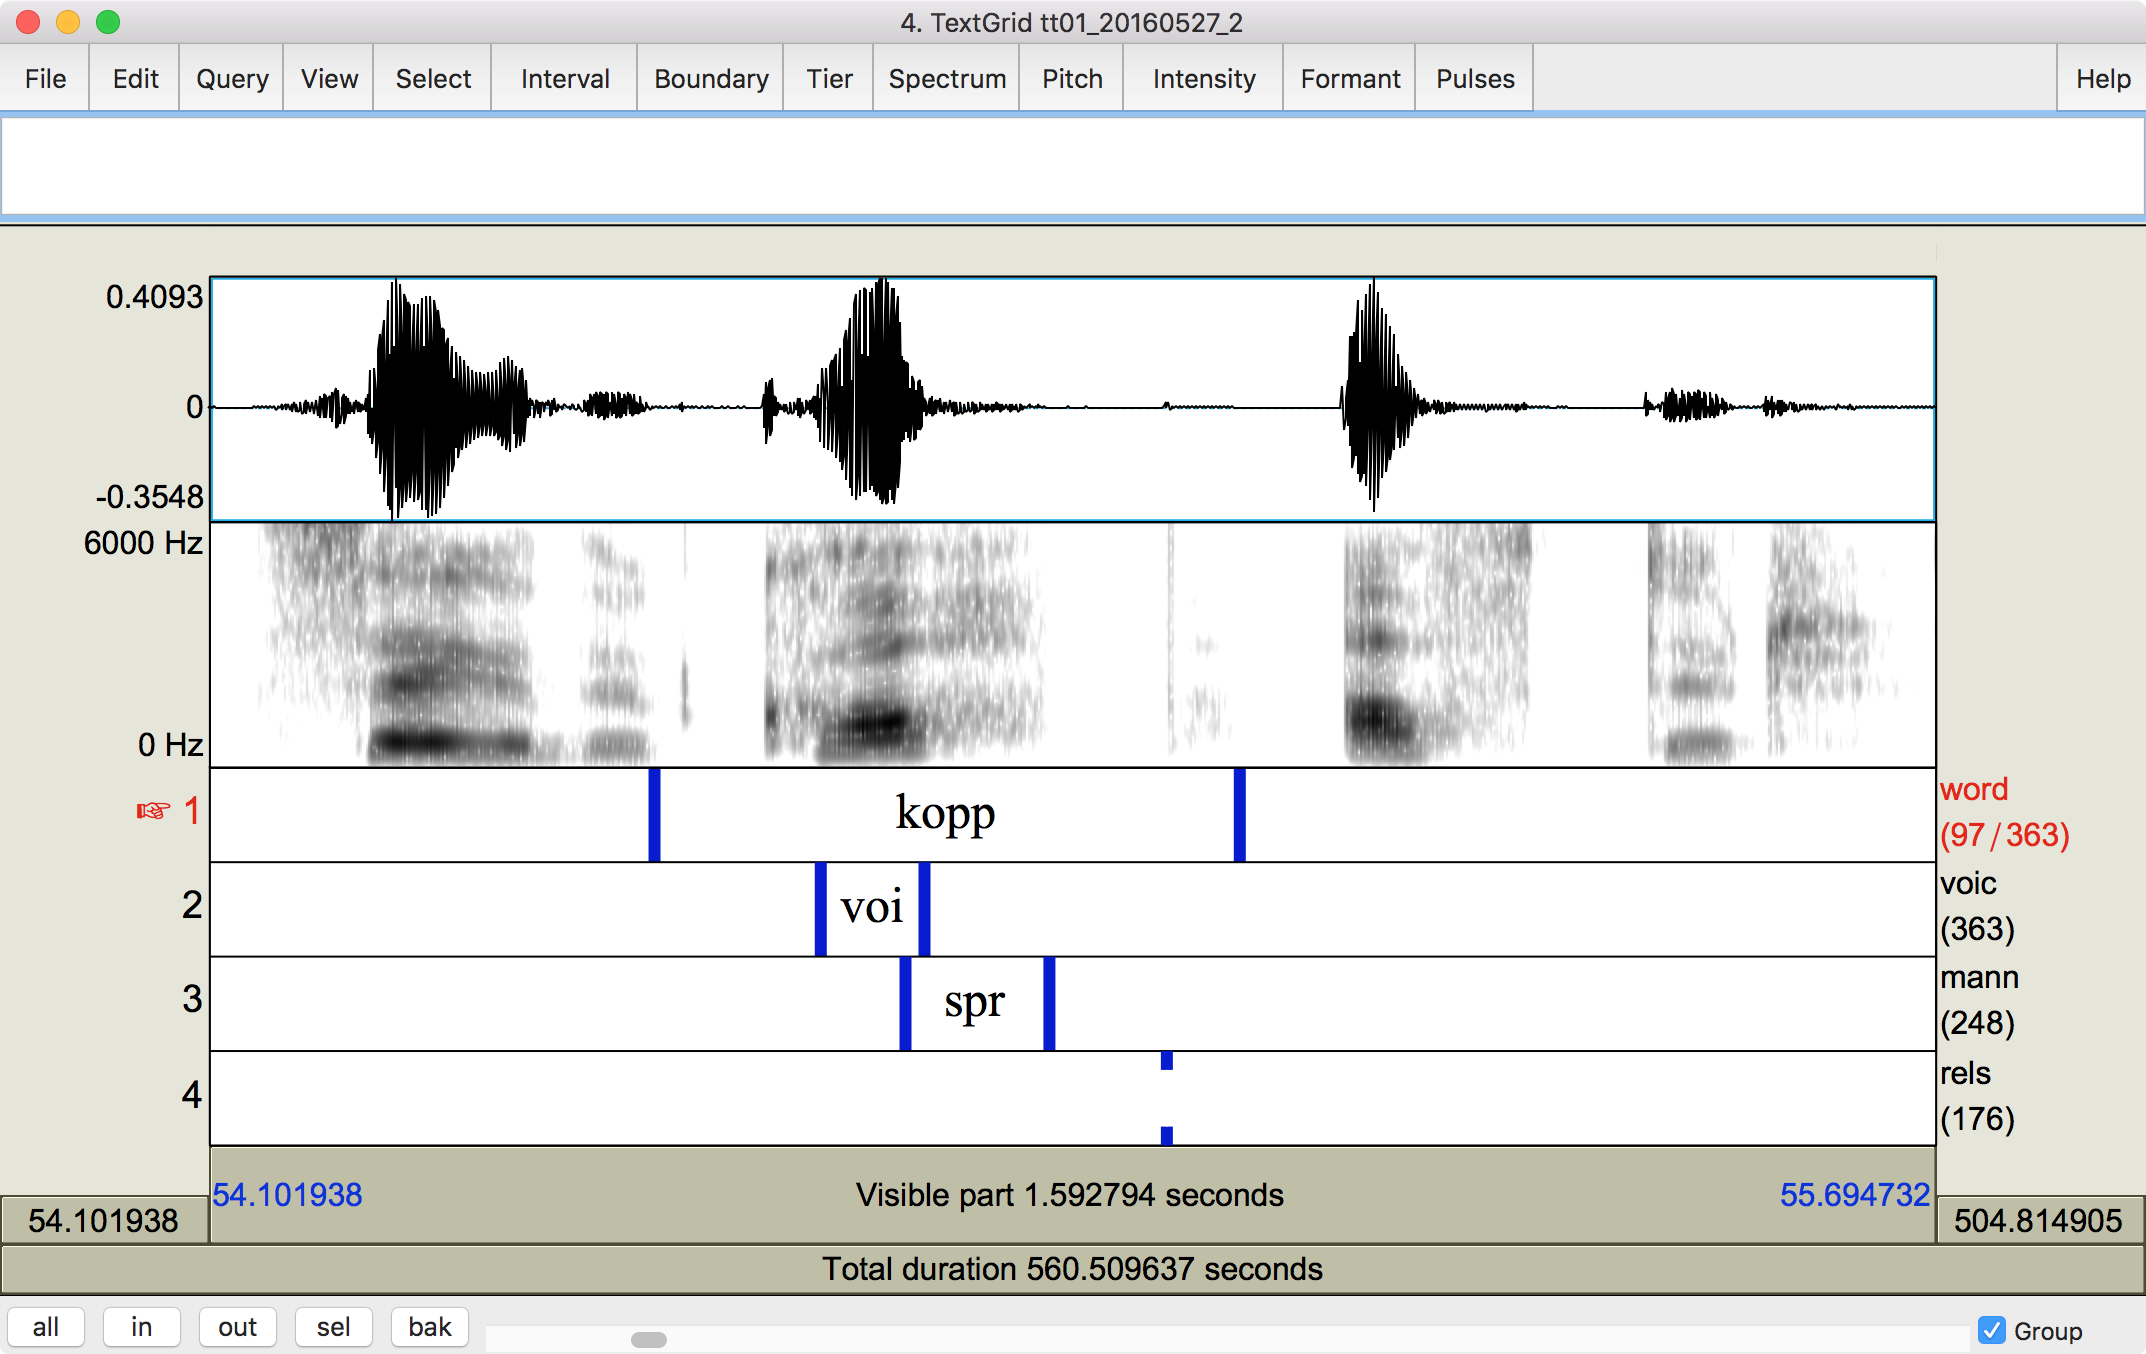
\includegraphics[width=\linewidth]{textgrid}
\caption{Example of the tier structure of the annotation files (PRAAT TextGrids).}
\label{f:textgrid}
\end{figure}

The analysis of the audio file consisted of three phases:
\begin{inparaenum}[(1)]
	\item conversion from stereo to mono,
	\item annotation, and
	\item extraction of measurements.
\end{inparaenum}
I first converted the audio files from stereo to mono, but I did not apply any filter.
During the second phase, I annotated the files in PRAAT \citep{boersma2015} using TextGrid files.
The annotation files have four tiers.
The tiers contain, respectively: 
\begin{inparaenum}[(1)]
	\item the graphemic transcriptions of the target words,
	\item the voiced intervals within the relevant portion of the words, 
	\item the intervals within the words where laryngeal spread, nasality, laterality or rhoticity is present, and
	\item the release of stops.
\end{inparaenum}
\Cref{f:textgrid} shows an example of the TextGrid set-up.

\subsection{Tier 1: words}

The first tier was segmented by target words.
The left boundary of the word was considered to be the off-set of voicing of the final vowel of \textit{segðu}, which preceded the target word.
The right boundary differed between consonant-final and vowel-final words.
In consonant-final words, the right boundary coincided with the end of the friction following the burst of the release, as visible in the waveform and spectrogram.
In vowel-final words, I used different criteria depending on the phonetic realisation.
The right boundary was placed at the off-set of voicing of the word-final vowel if followed by a pause; if the word-final vowel differed from the following and there was no pause, I placed the boundary at the mid-point of the transition between the final vowel and the initial vowel of the following word (\textit{aftur}); if a clear glottal stop separated the target word from the following, the boundary coincided with the on-set of the glottal stop.
In some cases, instead of a glottal stop, creaky voice was visible and the criterion of the transition mid-point was applied.

\subsection{Tier 2: voicing}

The second tier was reserved for the portions of vocal folds vibration (voicing).
The boundaries of the intervals in this tier were placed at the on-set and off-set of voicing around the target vowel.
In words starting with one or more voiced continuant consonants, the portion of voicing of those consonants was excluded from the interval and the left boundary was placed at the beginning of the vowel following the word-initial consonants.

\subsection{Tier 3: glottal spreading}

The third tier was used to annotate glottal spread, nasal airflow, laterality and rhoticity.
Marking the beginning of glottal spread proved to be particularly difficult.
The common realisation of the combination vowel + pre-aspiration is structured as follows: the first portion of the vocalic is accompanied by modal voicing; the glottis starts an abduction gesture while still vibrating the vocal folds (breathy voice); vocal fold vibration stops and voiceless friction remains (at the glottis or at the oral cavity, depending on the vowel).
%ADD glottal picture
As \citet{khan2012} and \citet{nance2013} point out, breathy voice is expected to produce more round-shaped periodic waves.
I took the onset of such more sinusoidal waves to coincide with glottal spread and I marked it as the left boundary of spreading.
However, at times the interpretation of the waveform was not straightforward.
In these cases, I relied on the visual make-up of the spectrogram.
According to \citet{jones2006} (cited in \citet[134]{nance2013}), breathy voice usually correlates with smeared off or totally absent higher formants.
This is due to the presence of high-frequency noise produced by the increased amount of airflow coming from the abducted glottis.
The right boundary was assumed to fall at the end of visible frication noise.

\subsection{Tier 3: nasals, laterals and rhotics}

Following standard practice, I marked the beginning of nasality where a change in the shape of the waveform and in the amplitude of the spectrogram were visible.
I applied the same principle to laterals and rhotics.
I placed the right boundary of these intervals (nasal, lateral, rhotic) depending on the voicing of the segment.
The voiceless nasal, lateral and trill consonants terminate with voiceless friction (nareal, lateral or central, respectively).
The end of friction in these consonants was used as the end of the interval.
In the voiced counterparts of these, the end of voicing coincided with the right boundary.
%ADD manner pictures

\subsection{Tier 4: consonant release}
In tier 4, the release of the stop consonant following the target vowel was marked at the onset of the burst.
If the burst was not visible in the waveform, no release was marked.

\section{Measurements}
%ADD put what you measured
In the third phase, I extracted the durational properties of the annotated intervals through an automated routine.
The routine was run with a PRAAT script, specifically written for this study.
The script with its documentation can be found in \Cref{a:getmeasure}.
The output is a \texttt{.csv} file with the relevant measurements.
The following measures were taken (all measures are in seconds):

\begin{itemize}
\item \textit{Word duration}: the duration of the whole word as annotated on tier 1
\item \textit{Duration of voicing}: the duration of the voicing interval on tier 2
\item \textit{Duration of manner}: the duration of the manner interval on tier 3 (this can be glottal spreading, nasality, laterality or the rhoticity)
\item \textit{Duration of absolute voicing}: this was measured as the duration of the interval between the onset of voicing and the onset of the manner interval, in words containing a pre-aspirated geminate or a sonorant (nasal or liquid); in words with non-aspirated geminates, the duration of absolute voicing is the same as the duration of voicing
\item \textit{Closure duration}: the duration of the stop closure, calculated as the duration of the interval between the off-set of voicing or, if present, manner and the release
\item \textit{Absolute closure duration}: the duration of the interval between the on-set of the manner and the release; in words with non-aspirated geminates, it is the same as the closure duration
\end{itemize}


\section{Statistical analysis}

I performed the statistical analysis using the R programming language \citep{r-core-team2015} in RStudio \citep{rstudio-team2015}.
















\chapter{Results}
\label{c:results}

\section{Word duration}


The word list used in the reading task contains both mono- and disyllabic words.
Both classes are further divided between consonant- and vowel-initial words.
It is thus sensible to report some of the measures for each class separately.
The mean duration of CVCC words is 441.36 msec (SD = 78.24), while for VCC is 338.71 msec (SD = 54.86).
CVCCV words have a mean duration of 488.55 msec (SD = 60.93), while VCCV are on average 424.99 msec long (SD = 53.42).

\begin{figure}
\centering
\begin{knitrout}
\definecolor{shadecolor}{rgb}{0.969, 0.969, 0.969}\color{fgcolor}
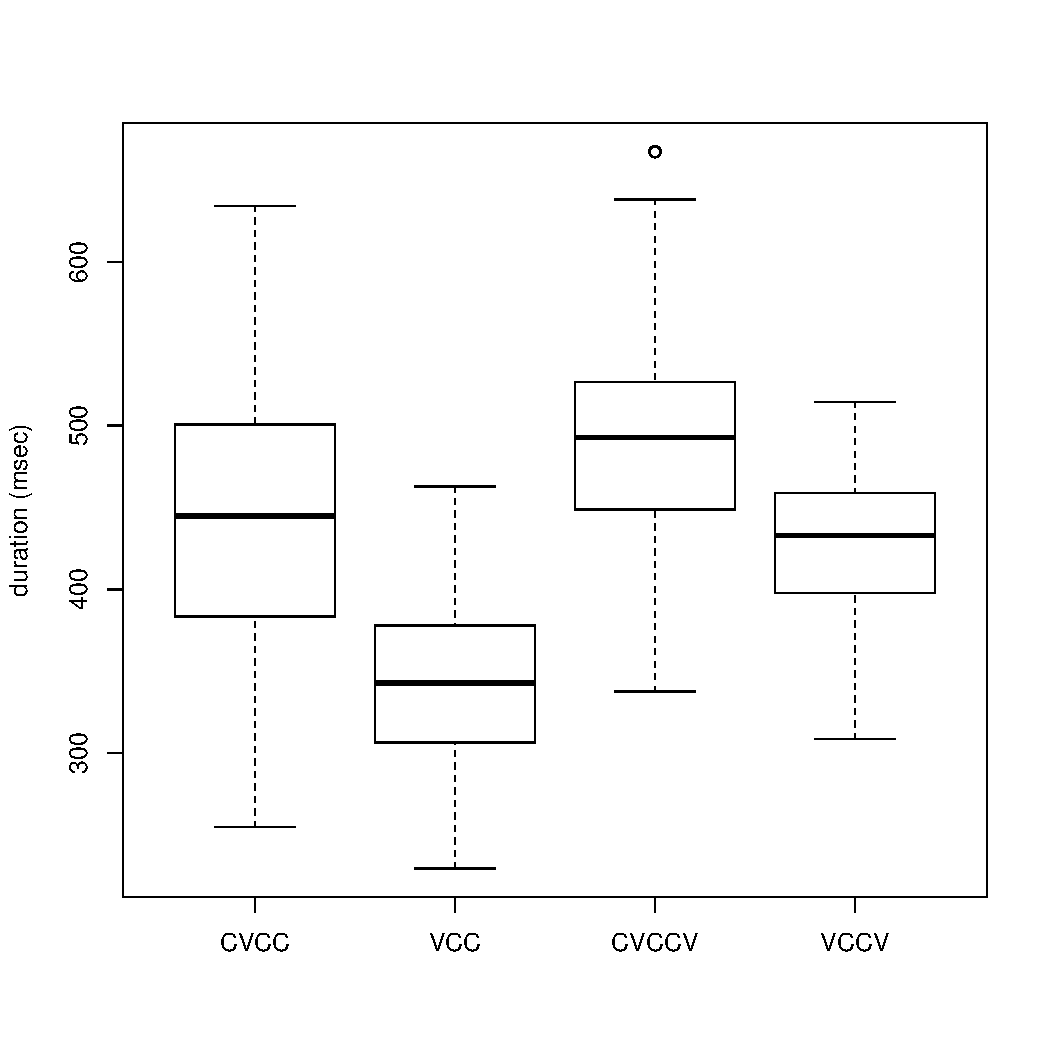
\includegraphics[width=0.6\textwidth]{img/word-duration-1} 

\end{knitrout}
\caption{Duration (in msec) of CVCC, VCC, CVCCV, and VCCV words.}
\label{f:worddur}
\end{figure}



% normalised voic is not different, but absolute is!, given that VOR is different, treat them differently
The duration of the voiced vocalic portion was not affected by the the number of syllables of the word.
The boxplot in \Cref{f:vvpsyll} shows the duration of the vocalic portion in milliseconds.
According to a two-sample Wilcoxon test, the mean duration of the voiced portion in monosyllabic words () does not different significantly from the mean duration in disyllabic words () [V = ].
However, the voice on-set to release was shorter in disyllabic words () than in monosyllabic words () [].
% kembt behave strange, in bte
Since duration normalisation was based on the voice on-set to release duration, in the next sections I will discuss monosyllabic and disyllabic words separately.

\section{Monosyllabic words}

\subsection{Geminate stops}



The mean duration of the voiced portion in milliseconds was 98 in words ending in a non-aspirated geminate stop, while it was 84.47 if followed by a pre-aspirated geminate stop.
\Cref{f:monostop} shows the normalised ratio of the voiced portion.
The difference in the mean of the normalised voiced ratio between the non-aspirated and the aspirated class of words was significant [].

\begin{figure}
\centering
\begin{knitrout}
\definecolor{shadecolor}{rgb}{0.969, 0.969, 0.969}\color{fgcolor}
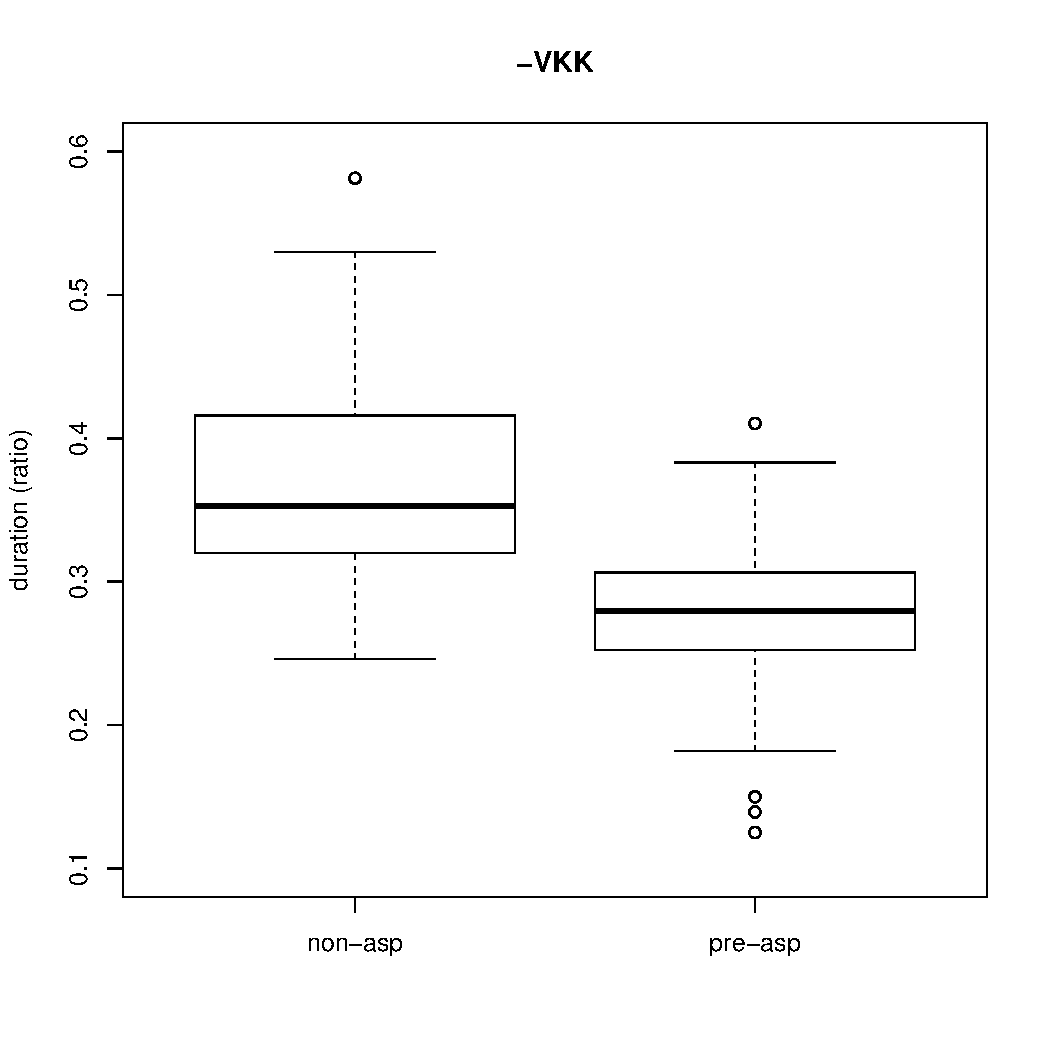
\includegraphics[width=0.6\textwidth]{img/mono-stop-box-1} 

\end{knitrout}
\caption{Duration (in ratios) of the voiced vocalic portion in geminate-final words.}
\label{f:monostop}
\end{figure}

\subsection{Nasals}



Words of the form (C)VNC showed a mean voiced portion duration of 98 msec if the nasal is voiced and 84.47 msec if voiceless.
The normalised duration was, respectively, 0.37 and 0.28.

\subsection{Laterals}



In the case of words ending in a /lC/ cluster, the mean duration of the vocalic portion were 102.05 and 80.7 msec when followed, respectively by a voiced and voiceless lateral.
These correspond to the 29.69\% and the 24.98\% of the VOR.
A Wilcoxon test shows that the difference is significant [].

\section{Disyllabic words}

\subsection{Geminate stops}




In disyllabic words, the voiced vocalic portion is 86.97 msec long if followed by a non-aspirated geminate, and 78.04 msec long if followed by a pre-aspirated geminate.
In ratio terms, the voiced part makes up the 33.61\% of the VOR in word with plain geminates, and the 28.27\% in words with pre-aspirated geminates.
According to a independent two-sample \textit{t}-test, the difference in ratio is significant.

\subsection{Nasals}




CVNCV words have a mean voiced vocalic portion duration of 81.72 msec if the nasal is voiced and 67.83 msec if it is voiceless.
As percentages, the vocalic portion is 29.47\% of the VOR if followed by a voiced nasal, and 24.22\% when the nasal is voiceless.
A \textit{t}-test showed that this difference is significant.

\subsection{Laterals}



The voiced vocalic portion in CVLCV words is on average 107.68 msec long when the lateral is voiced and 66.66 msec when it is voiceless.
The voiced portion takes the 36.2\% of the VOR if followed by a voiced lateral, and 23.26\% when the lateral is voiceless.


\subsection{Rhotics}



With words containing an /rC/ cluster, the mean duration of the voiced vocalic portion is 121.07 msec long when the rhotic is voiced and 104.78 msec when it is voiceless.
The voiced portion takes the 39.83\% of the VOR if followed by a voiced rhotic, and 33.43\% when the rhotic is voiceless.








\chapter{Discussion}

The research hypothesis of this study is based on the idea that the aspiration effect could be the product of the relative timing of the glottal spread gesture in relation to the tongue gestures in the oral cavity.
An early timing of glottal spread would shorten the vowel, while a later timing would lengthen it.
In particular, the hypothesis states that, in Icelandic, vowels followed by aspirated consonants (pre-aspirated geminates and voiceless sonorants) should be shorter than vowels followed by plain consonants.
As shown in the result chapter (\Cref{c:results}), I found a significant difference between the duration of the voiced vocalic portion in words with aspirated consonants and its duration in words with non-aspirated consonants.
This finding seems to support the timing hypothesis.

\section{Geminate stops}
%ADD many figures
We have seen that the absolute duration of vowels is smaller when they are followed by a pre-aspirated geminate than when they are followed by a plain geminate.
It is worth noting that the VOR of the two classes is different, as said in .
However, the fact that the vowel is shorter in words with pre-aspirated geminates cannot be attributed to differences in the over-all duration of the interval between the onset of voicing and the release of the stop.
This is because the VOR is \textit{longer} in words with aspiration while the absolute duration of the vowel is \textit{smaller}.
Other things being equal, we would expect the interval between voice onset and the onset of glottal abduction in words with pre-aspiration to take the same ratio of the VOR as the voiced interval in words with plain geminates.
Instead, laryngeal spreading starts quite early in the word, while voicing is still active even after glottal spread is initiated.

It can be then argued that the relative earlier timing of glottal abduction reduces the vocalic portion where modal voicing is maintained.
This kind of alignment results in a shorter vowel, if we consider the vowel to be the modal voiced interval of the vocalic gesture.
Moreover, when breathy voicing (which is voicing with concomitant abducted vocal folds) is visible from the spectrogram, it should be assumed that the spreading gesture has reached the critical point where the abduction is enough to produce breathiness.
This would imply that the gestured might start even earlier, strengthening the central idea proposed in this research.

However, the hypothesis rested on the idea that voicing would cease earlier in vowels followed by pre-aspirated stops, resulting in a shortened vowel.
What I found, instead, points to a longer voicing portion in words with pre-aspirated stops.
The duration of voicing is, in fact, greater in words with pre-aspirated stops than in word with plain geminates.
This is not surprising, since glottal spread is not incompatible with voicing and could actually allow voicing to be maintained longer.
A plain geminate is produced by keeping the closure for a longer time and voicing during closure is more difficult to maintain.
Thus it is natural to expect that, other things being equal, voicing duration would be greater if glottal spread is involved.
This fact does not fit well with the idea that voicing should cease earlier due to glottal spread.
Even if the physiological explanation seems not to hold, the relative timing on itself can be provisionally considered to be right.

\begin{figure}
\centering
\begin{knitrout}
\definecolor{shadecolor}{rgb}{0.969, 0.969, 0.969}\color{fgcolor}
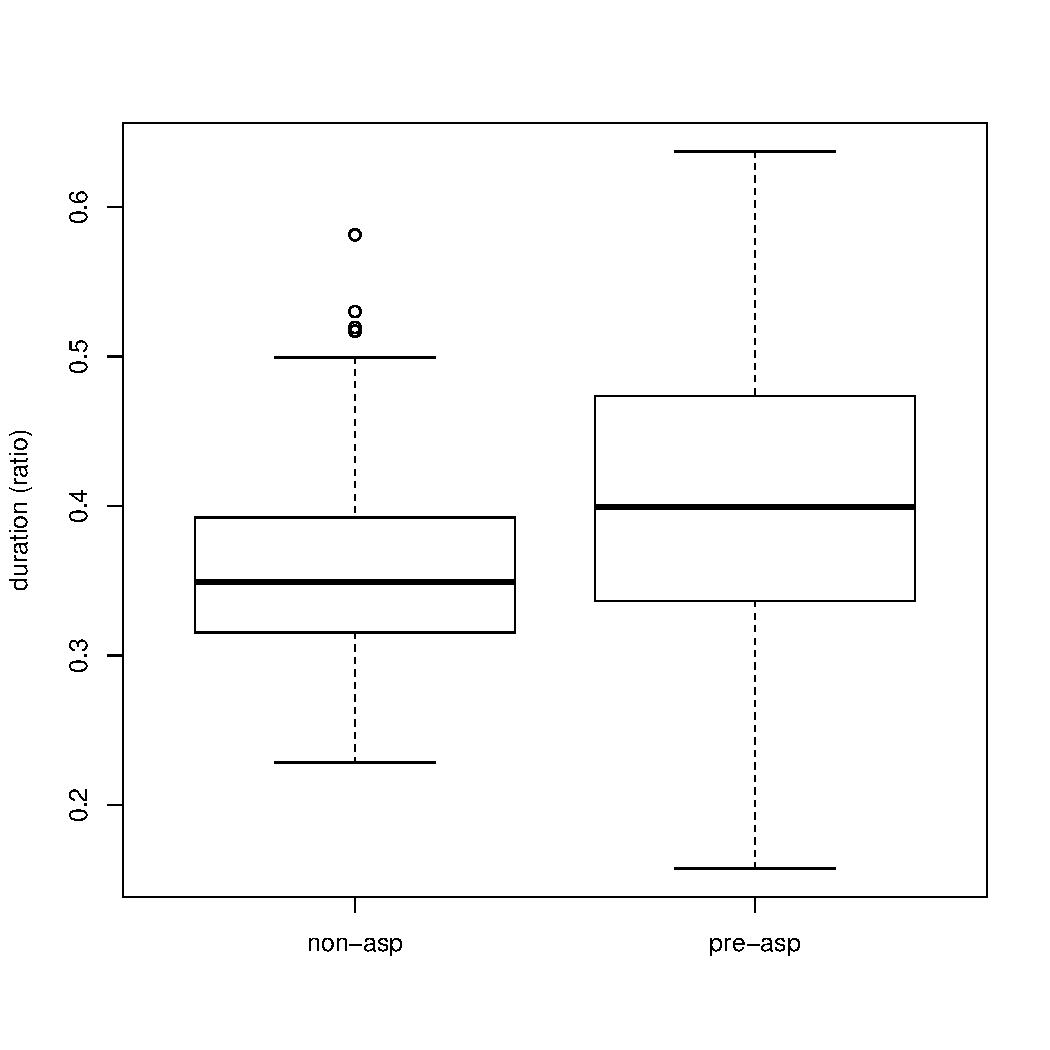
\includegraphics[width=0.6\textwidth]{img/voic-stop-1} 

\end{knitrout}
\caption{Ratio duration of the voicing interval depending on presence or absence of glottal spread.}
\label{f:voicdur}
\end{figure}

Contrary to what stated in \Cref{s:hypothesis}, glottal abduction does not prevent voicing.
On the contrary, longer voicing can be found in words with glottal spread.
A possible explanation of this phenomenon is that the absence of a closure at the VC transition allows for voicing to continue.
In words without gottal spread, the closure of the plain geminate---which is produced immediately after the vowel---quickly produces an increas in oral pressure, until the point is reached when voicing can no longer be sustained.
At the same time, the variance of voicing in the two classes is not the same, and voicing in the aspirated condition has greater variance.
In some aspirated tokens, the duration of voicing is as short---or in a few cases even shorter--- than the duration in non-aspirated tokens.

\section{Sonorants}




\section{Limitations and further studies}









%\chapter{Conclusion}

\appendix


\chapter{Word list}
\label{a:list}


\ctable[caption = List of target words,
label = t:target
]{cccc}{}{
\FL
word  & IPA    & word   & IPA     \ML
kokk  & kʰoʰk  & kembt  & kem̥t    \NN
gogg  & kokk   & kembdi & kemtɪ    \NN
dökk  & tœʰk   & kampa  & kʰam̥pa  \NN
dögg  & tœkk   & kamba  & kʰampa   \NN
kopp  & kʰoʰp  & kempa  & kʰem̥pa  \NN
kubb  & kʰʏpp  & kemba  & kʰempa   \NN
vítt  & viʰt   & punta  & pʰʏn̥ta  \NN
vídd  & vitt   & punda  & pʰʏnta   \NN
þítt  & θiʰt   & vanta  & van̥ta   \NN
þíddi & θittɪ  & vanda  & vanta    \NN
fætt  & faiʰt  & fínn   & fitn̥    \NN
fæddi & faittɪ & kinn   & kʰɪnn    \NN
ýtt   & iʰt    & duld   & tʏlt     \NN
ydd   & ɪtt    & dult   & tʏl̥t    \NN
ótt   & ouʰt   & gelta  & kel̥ta   \NN
odd   & ott    & gelda  & kelta    \NN
sets  & sess   & orka   & or̥ka    \NN
sett  & seʰt   & orga   & orka     \NN
feits & feiss  & mjólka & mjoul̥ka \NN
feitt & feiʰt  & ólga   & oulka    \NN
vots  & voss   & hefna  & hepna    \NN
vott  & voʰt   & vopna  & voʰpna   \NN
takka & tʰaʰka & nafla  & napla    \NN
kagga & kʰakka & japla  & jaʰpla   \NN
detta & teʰta  & kafli  & kaplɪ    \NN
gedda & ketta  & kapli  & kaʰplɪ   \NN
kamp  & kʰam̥p & tefla  & tepla    \NN
kamb  & kʰamp  & tipla  & tɪʰpla   \NN
punt  & pʰʏn̥t &        &          \NN
pund  & pʰʏnt  &        &         \LL
}





\chapter{PRAAT script}
\label{a:getmeasure}








\bibliographystyle{york-harvard}
\bibliography{linguistics}

\end{document}
